\documentclass[tikz,border=8pt]{standalone}
\usepackage{amsmath}
\usetikzlibrary{arrows.meta,calc,decorations.pathmorphing}
\definecolor{ink}{HTML}{21352F}
\definecolor{teal}{HTML}{087F7B}
\definecolor{gold}{HTML}{C58B2A}
\definecolor{blue}{HTML}{4B77A8}
\definecolor{rose}{HTML}{B65A62}
\begin{document}
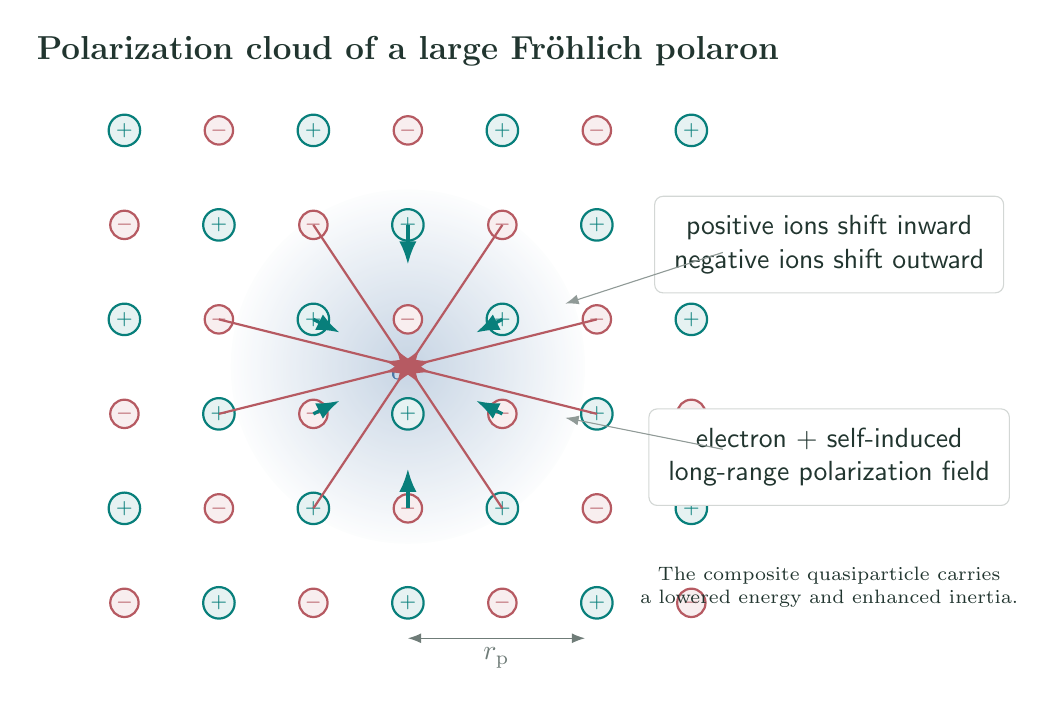
\begin{tikzpicture}[font=\sffamily,text=ink,>=Latex]
  \node[font=\bfseries\large] at (0,4.0) {Polarization cloud of a large Fr\"ohlich polaron};
  \shade[inner color=blue!42,outer color=blue!2,opacity=.75] (0,0) circle (2.25);
  \node[blue,font=\bfseries\large] at (0,0) {$e^-$};
  \foreach \x in {-3.6,-2.4,-1.2,0,1.2,2.4,3.6}{
    \foreach \y in {-3.0,-1.8,-0.6,0.6,1.8,3.0}{
      \pgfmathtruncatemacro{\parity}{mod(round((\x+3.6)/1.2)+round((\y+3.0)/1.2),2)}
      \ifnum\parity=0
        \draw[rose,thick,fill=rose!10] (\x,\y) circle (0.18);
        \node[rose,font=\scriptsize] at (\x,\y) {$-$};
      \else
        \draw[teal,thick,fill=teal!10] (\x,\y) circle (0.20);
        \node[teal,font=\scriptsize] at (\x,\y) {$+$};
      \fi
    }
  }
  \node[blue,font=\bfseries\large] at (0,0) {$e^-$};
  \foreach \x/\y in {-1.2/-0.6,1.2/-0.6,-1.2/0.6,1.2/0.6,0/-1.8,0/1.8}{
    \draw[->,teal,very thick] (\x,\y)--($(\x,\y)!0.28!(0,0)$);
  }
  \foreach \x/\y in {-2.4/-0.6,2.4/-0.6,-2.4/0.6,2.4/0.6,-1.2/-1.8,1.2/-1.8,-1.2/1.8,1.2/1.8}{
    \draw[->,rose,thick] (\x,\y)--($(0,0)!-0.12!(\x,\y)$);
  }
  \draw[<->,ink!65] (0,-3.45)--(2.25,-3.45) node[midway,below] {$r_{\rm p}$};
  \node[draw=ink!20,rounded corners=3pt,fill=white,inner sep=7pt,align=center] at (5.35,1.55) {positive ions shift inward\\negative ions shift outward};
  \draw[->,ink!50] (4.0,1.45)--(2.0,0.8);
  \node[draw=ink!20,rounded corners=3pt,fill=white,inner sep=7pt,align=center] at (5.35,-1.15) {electron $+$ self-induced\\long-range polarization field};
  \draw[->,ink!50] (4.0,-1.05)--(2.0,-0.65);
  \node[font=\scriptsize,align=center] at (5.35,-2.8) {The composite quasiparticle carries\\a lowered energy and enhanced inertia.};
\end{tikzpicture}
\end{document}
